\subsection{Three Minute Thesis}
\label{subsec:3mt}

The Three Minute Thesis (3MT) is an academic research communication competition.
It celebrates the research conducted by graduate students, while challenging them to effectively explain the research---in spoken words in three minutes---in a language appropriate to a non-specialist audience.
Competitors are expected to have one static illustrative slide.
The 3MT competition has been organized annually at Augusta University since 2017.
I participated in the competition in 2024 with the following presentation.


\subsubsection{Smashing Software Bugs with Proofs}

We live in a world where software is everywhere. It wasn’t always so. When I was little, my parents had a push-button telephone and “updating a TV” meant buying a new one from a store. But we continue to experience fast exciting transformation with technology. However, the more software we come across, the more bugs we see. A bug is a fault in software that causes incorrect or unexpected behavior. Since we depend heavily on software, there is a high incentive to eliminate bugs. This is especially true for critical systems like cars and airplanes. Unfortunately, eliminating bugs is not easy. There are multiple challenges. Fundamentally, software is made of 0s and 1s. Even a simple computer has more ways to arrange the 0s and 1s than there are atoms in the universe. It is impossible to test everything. Software engineers are under pressure to publish releases, so quality control steps get overlooked.

I research ways to reduce these challenges. I want to empower software engineers to build high quality correct applications. The strategy is to build specialized software, called verifiers, to check other software. But if we use software to verify software, what is there to say the verifier is correct? Answering this question is my research topic. See, I have a technique for software verification. It allows me to check that memory usage doesn’t get out of control. But to trust this technique, I have to prove it gives correct results. I do this by building mathematical proofs. But instead of pen and paper, I use a computer. First, I define a model. Then, I construct proofs about the model. I put those proofs together, like lego blocks, to form an even big proof. I can also check the proofs with a computer. These kind of mechanized proofs are the most rigorous ways we know for asserting correctness.

If I can complete my proof, it shows that achieving strong correctness guarantees is possible. It would enable building verifiers we can trust, and those would help software engineers eliminate bugs that impact us all. But there is an even more extended impact. Remember, everything in tech moves fast. Only this month we were introduced to the world’s first AI software engineer. You see, in their infinite wisdom the software engineers decided that software engineers should be among the first jobs replaced by AI. Talk about job security! But all software, whether created by humans or AI, need quality control checks. If we replace the human, we only have an increasing urgency for the techniques I am researching.

\begin{figure}[tb]
    \centering
    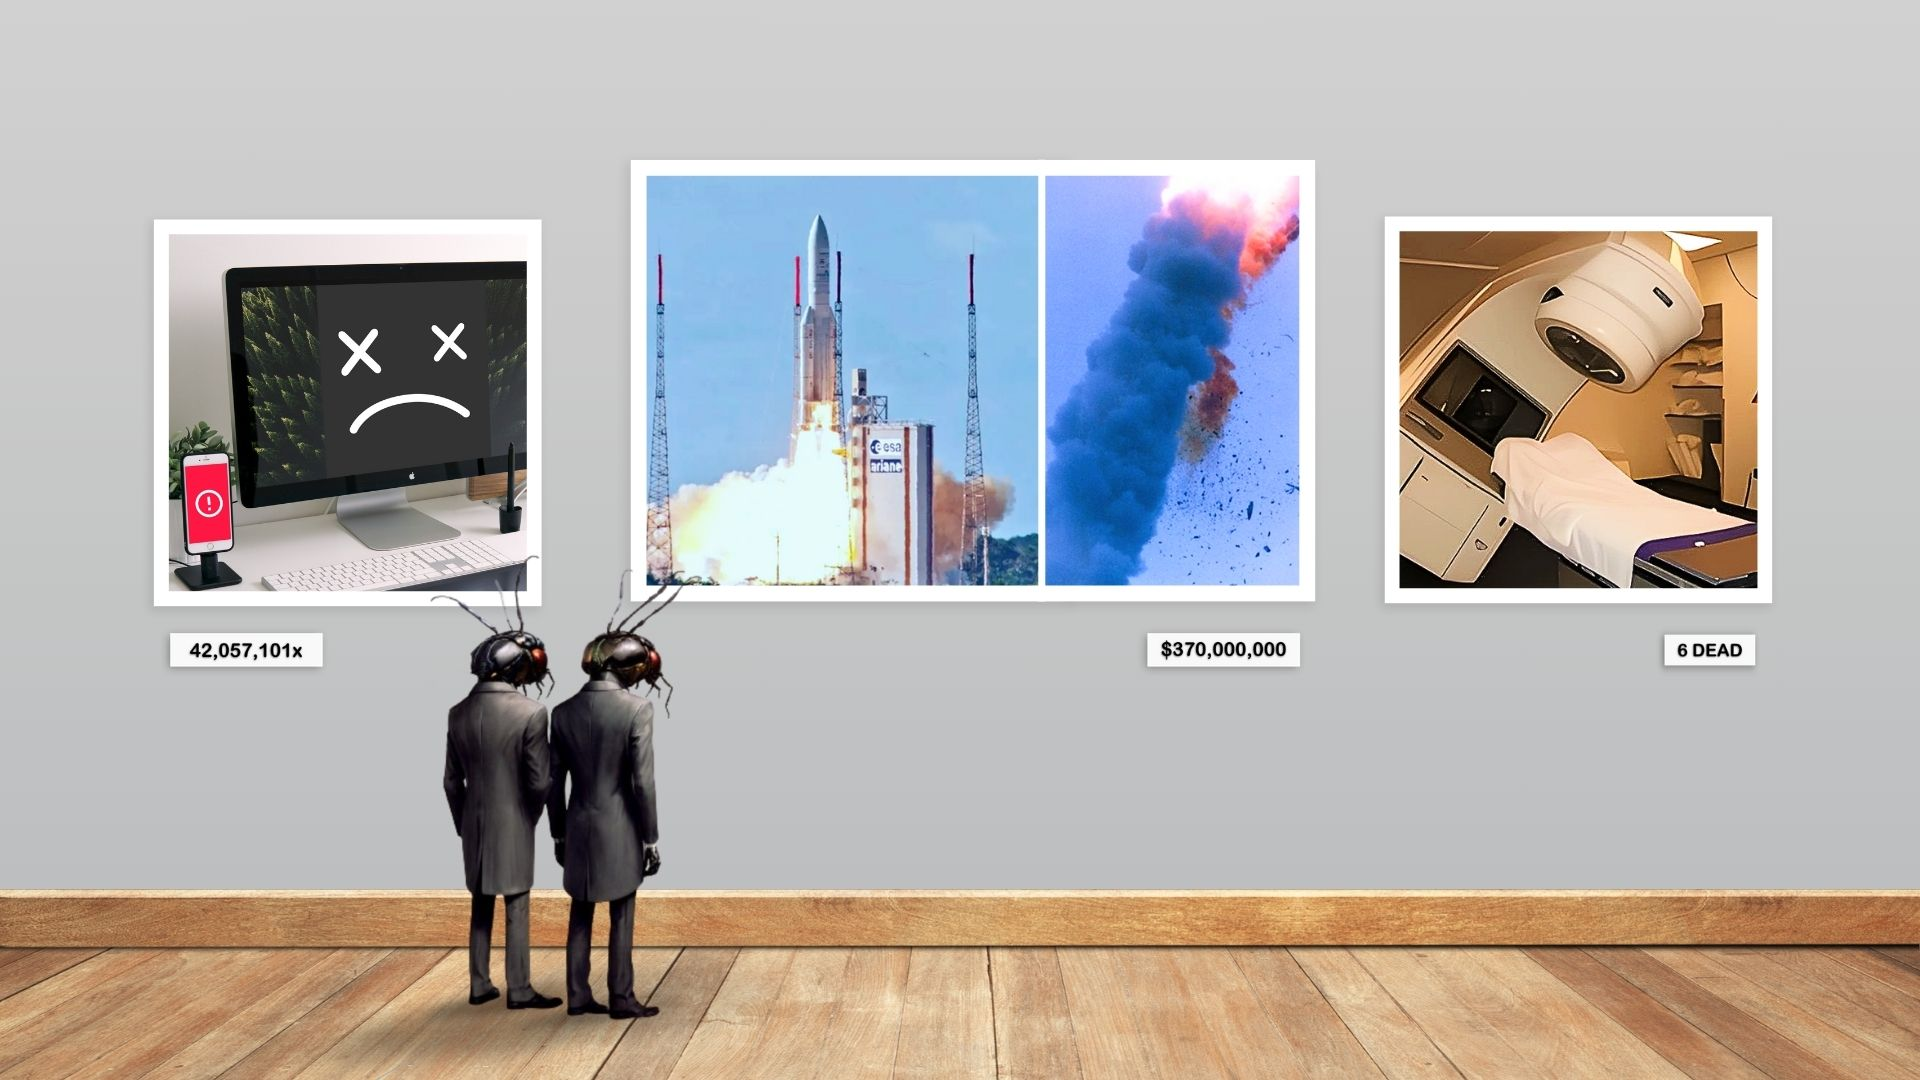
\includegraphics[width=\columnwidth]{img/3mt.jpg}
    \caption{3MT competition slide, \enquote{Smashing Software Bugs with Proofs}.}
    \label{fig:3mt-slide}
\end{figure}